\section*{Introducción}
En aplicaciones en las cuales se busca una respuesta certera y/o salida muy cercana a un valor deseado es necesario para tal propósito considerar dentro del modelo propuesto el tensión de offset que los amplificadores operacionales añaden a su salidan alterando según esta medida la respuesta de un sistema, es en tal sentido que surge la necesidad de medir  estas variaciones y corregirlas para restablecer un comportamiento adecuado del dispositivo.

En el presente informe se describe el procedimiento y componentes a considerar para la medición del voltaje de offset el cual eleve o decrementa una señal respecto a la referencia de 0v, utilizando para ello durante el experimento los amplificadores operacionales LM741 y TL081.

\section{Medición tensión eficaz (AC) y componente continua (DC)}

Para la medición de estos parámetros se hizo uso del multímetro digital disponible en el laboratorio perteneciente al modelo 2110 de la marca Keithley, para ello se tomo como referencia la hoja de datos de este dispositivo y el esquema de conexión para la medición de voltaje como se muestra en la figura \ref{fig:configuracion-multimetro}

\begin{figure}[h]
	\centering
	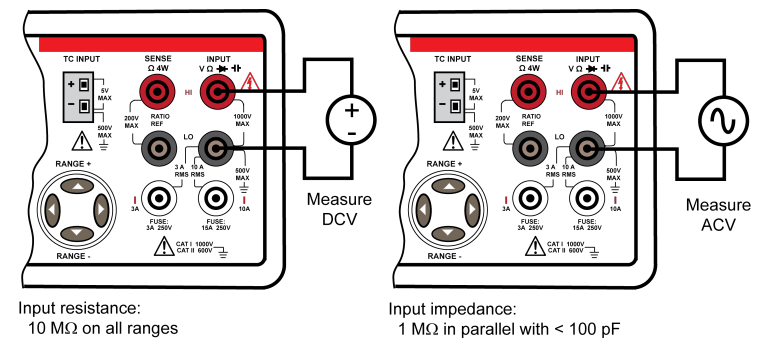
\includegraphics[width=0.5\textwidth]{media/configuracion-multimetro}
	\caption{Configuración Multimetro Keithley 2110}
	\label{fig:configuracion-multimetro}
\end{figure}

En la mediciones realizadas se obtuvieron valores determinados en la guía, siendo estos cercanos a 1.4140mV y 0v para las componentes AC y DC respectivamente.

\section{Tensión continua y efecto del condensador $C_1$ y resistencia $R_1$}

Al trabajarse con señales alternas durante el experimentación una medición DC en la resistencia $R_1$ tiene como resultado un valor de 0v, sin embargo al realizar esta misma medición para una configuración AC en el multímetro el capacitor $C_1$ y $R_1$ al tratarse de una reactancia capacitiva y la resistencia en la salida, tal topología actúa como un divisor de tensión, siendo para una frecuencia en la señal de entrada de 1k [Hz], se aprecia en la resistencia $R_1$ más del 70\% del voltaje defino en la entrada, siendo así que este nivel de voltaje es el aplicado en el amplificador operacional.

\section{Señal de entrada en la resistencia $R_1$}

Una vez configurado el instrumento de medición (osciloscopio) se procedió a realizar la conexión de la sonda entre los terminales de la resistencia, siendo estos próximos o similares a la señal alterna de entrada debido a la configuración como divisor de tensión explicada en el punto anterior, por lo tanto para esta mediciones se obtuvieron:

\begin{itemize}
	\item Amplitud: 20mVp
	\item Frecuencia: 1K Hz
	\item Valor medio (DC) : 0v
\end{itemize}

Sin embargo es necesario acotar que debido al excedo de ruido visto en la señal sinusoidal de 2 mVp para la experimentación, se trabajo con una señal de 20 [mVp] la cual corresponde con la señal medida en la entrada y un valor de 10.3120 [mVp] en la resistencia $R_1$.

\section{Características de la señal de salida - OPAM}

Para una medición en la señal de salida se hizo uso del pin 6 el cual es un terminal común que comparten los integrados tal y como se muestra en la hoja de datos para cada operacional a usar durante la experiencia, un resumen de esta especificación se muestra en las figuras \ref{fig:encapsulado-741} y \ref{fig:encapsulado-081} respectivamente.


\begin{figure}[h]
	\centering
	\begin{minipage}{0.4\linewidth}
		\centering	
		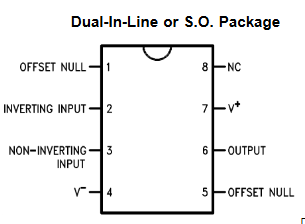
\includegraphics[width=\linewidth]{media/encapsulado-741}
		\caption{Encapsulado y pinout - LM741}
		\label{fig:encapsulado-741}	
	\end{minipage}
	\hfill
	\begin{minipage}{0.4\linewidth}
		\centering
		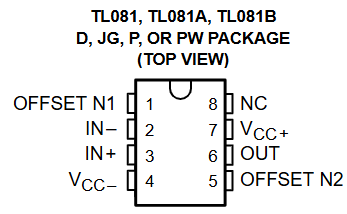
\includegraphics[width=\linewidth]{media/encapsulado-081}
		\caption{Encapsulado y pinout - TL081}
		\label{fig:encapsulado-081}
	\end{minipage}
	\caption{Pinout - Amplificadores Operacionales}
	\label{fig:integrados-opam}
\end{figure}

Finalmente las mediciones de la señal de salida se obtuvieron en el segundo terminal del osciloscopio (señal de color celeste) cuyos valores de voltaje fueron:

\begin{itemize}
	\item Amplitud: 1.44 Vp
	\item Valor medio: 211mV
	\item Frecuencia: 1K Hz
	\item Valor RMS: 1.03V
\end{itemize}

\subsection{¿Qué se observa de particular en la señal?}
En la señal de salida una peculiaridad es la comprobación de forma indirecta el nivel offset o nivel DC en la salida del operacional el cual tiene como causa un valor medio diferente a 0v; comprobando tales valores en la figura \ref{fig:salida-operacional}

\begin{figure}[h]
	\centering
	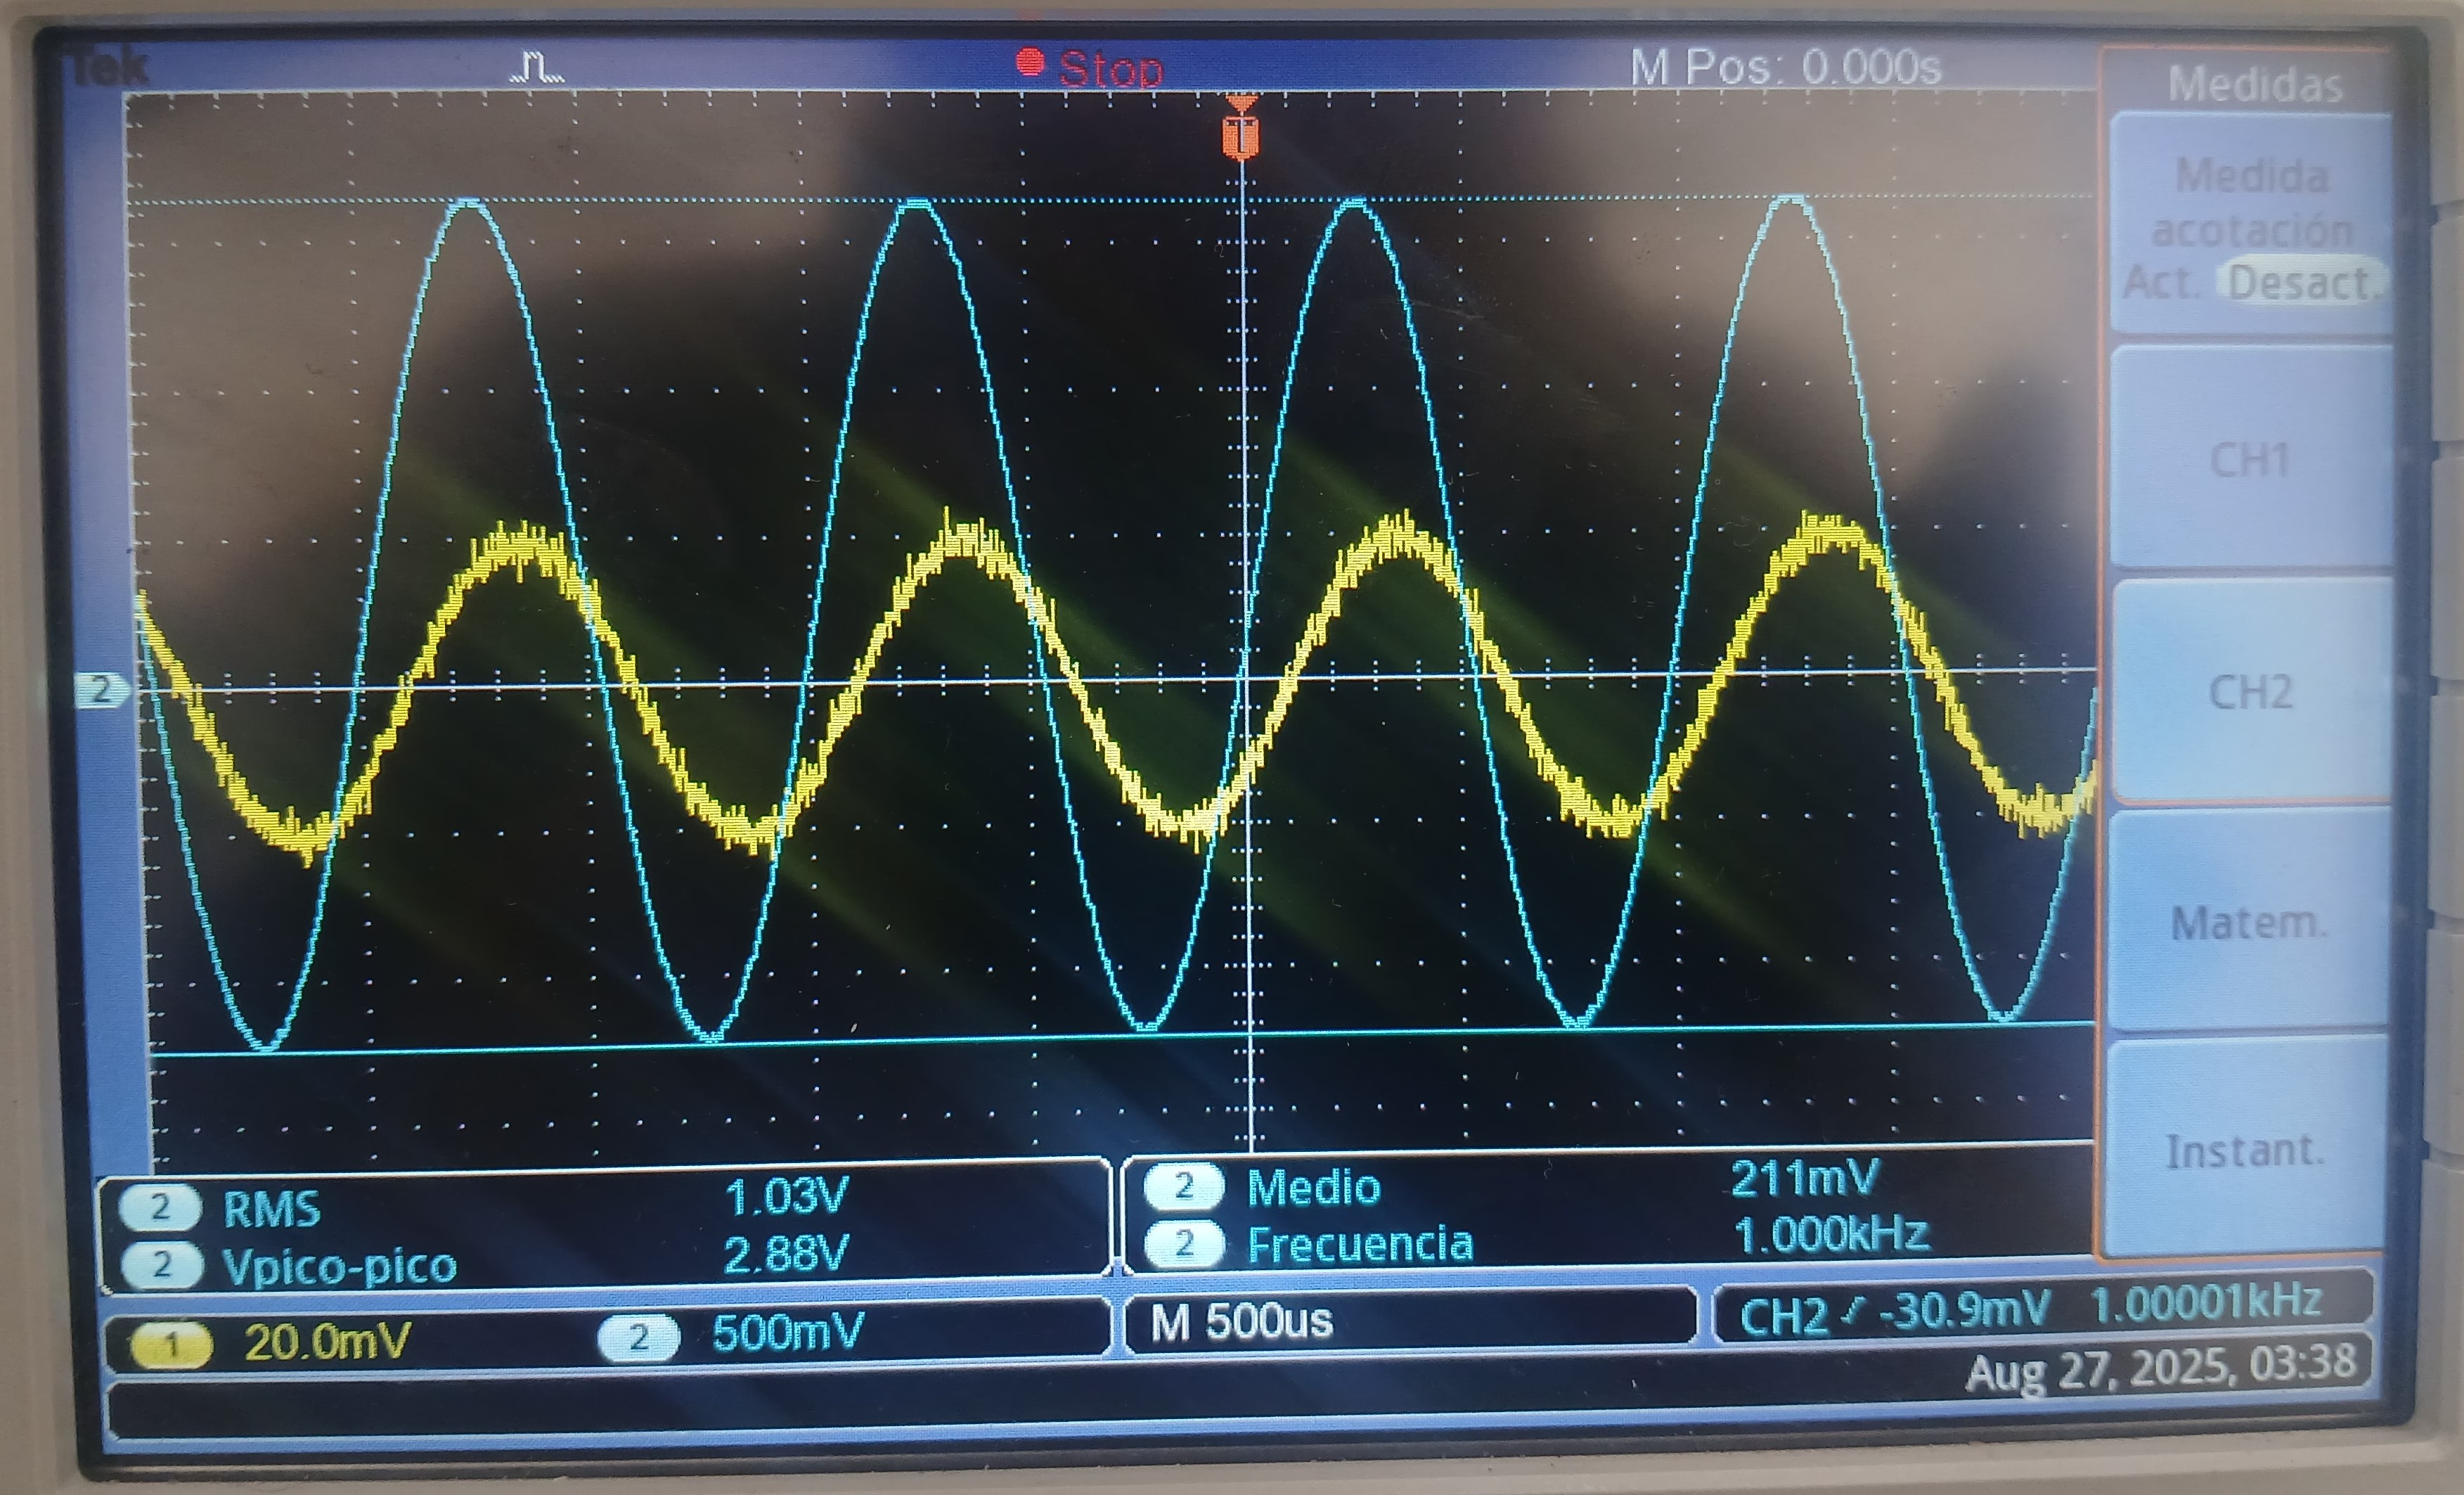
\includegraphics[width=0.5\textwidth]{media/salida-operacional}
	\caption{Señal de salida - Amplificador Operacional}
	\label{fig:salida-operacional}
\end{figure}

\section{Estimación del nivel de offset en el amplificador operacional}

Una forma de medir los niveles de voltaje en una señal alterna, como la determinación de valores pico es mediante el uso de cursores, siendo así que al asumir una señal senoidal simétrica ambos valores pico deberían corresponderse para el ciclo positivo y negativo en magnitud, por lo tanto en caso las mediciones no cumplan con esta condición se puede asumir la existencia de un valor DC u offset en la señal alterna.

\begin{figure}[h]
	\centering
	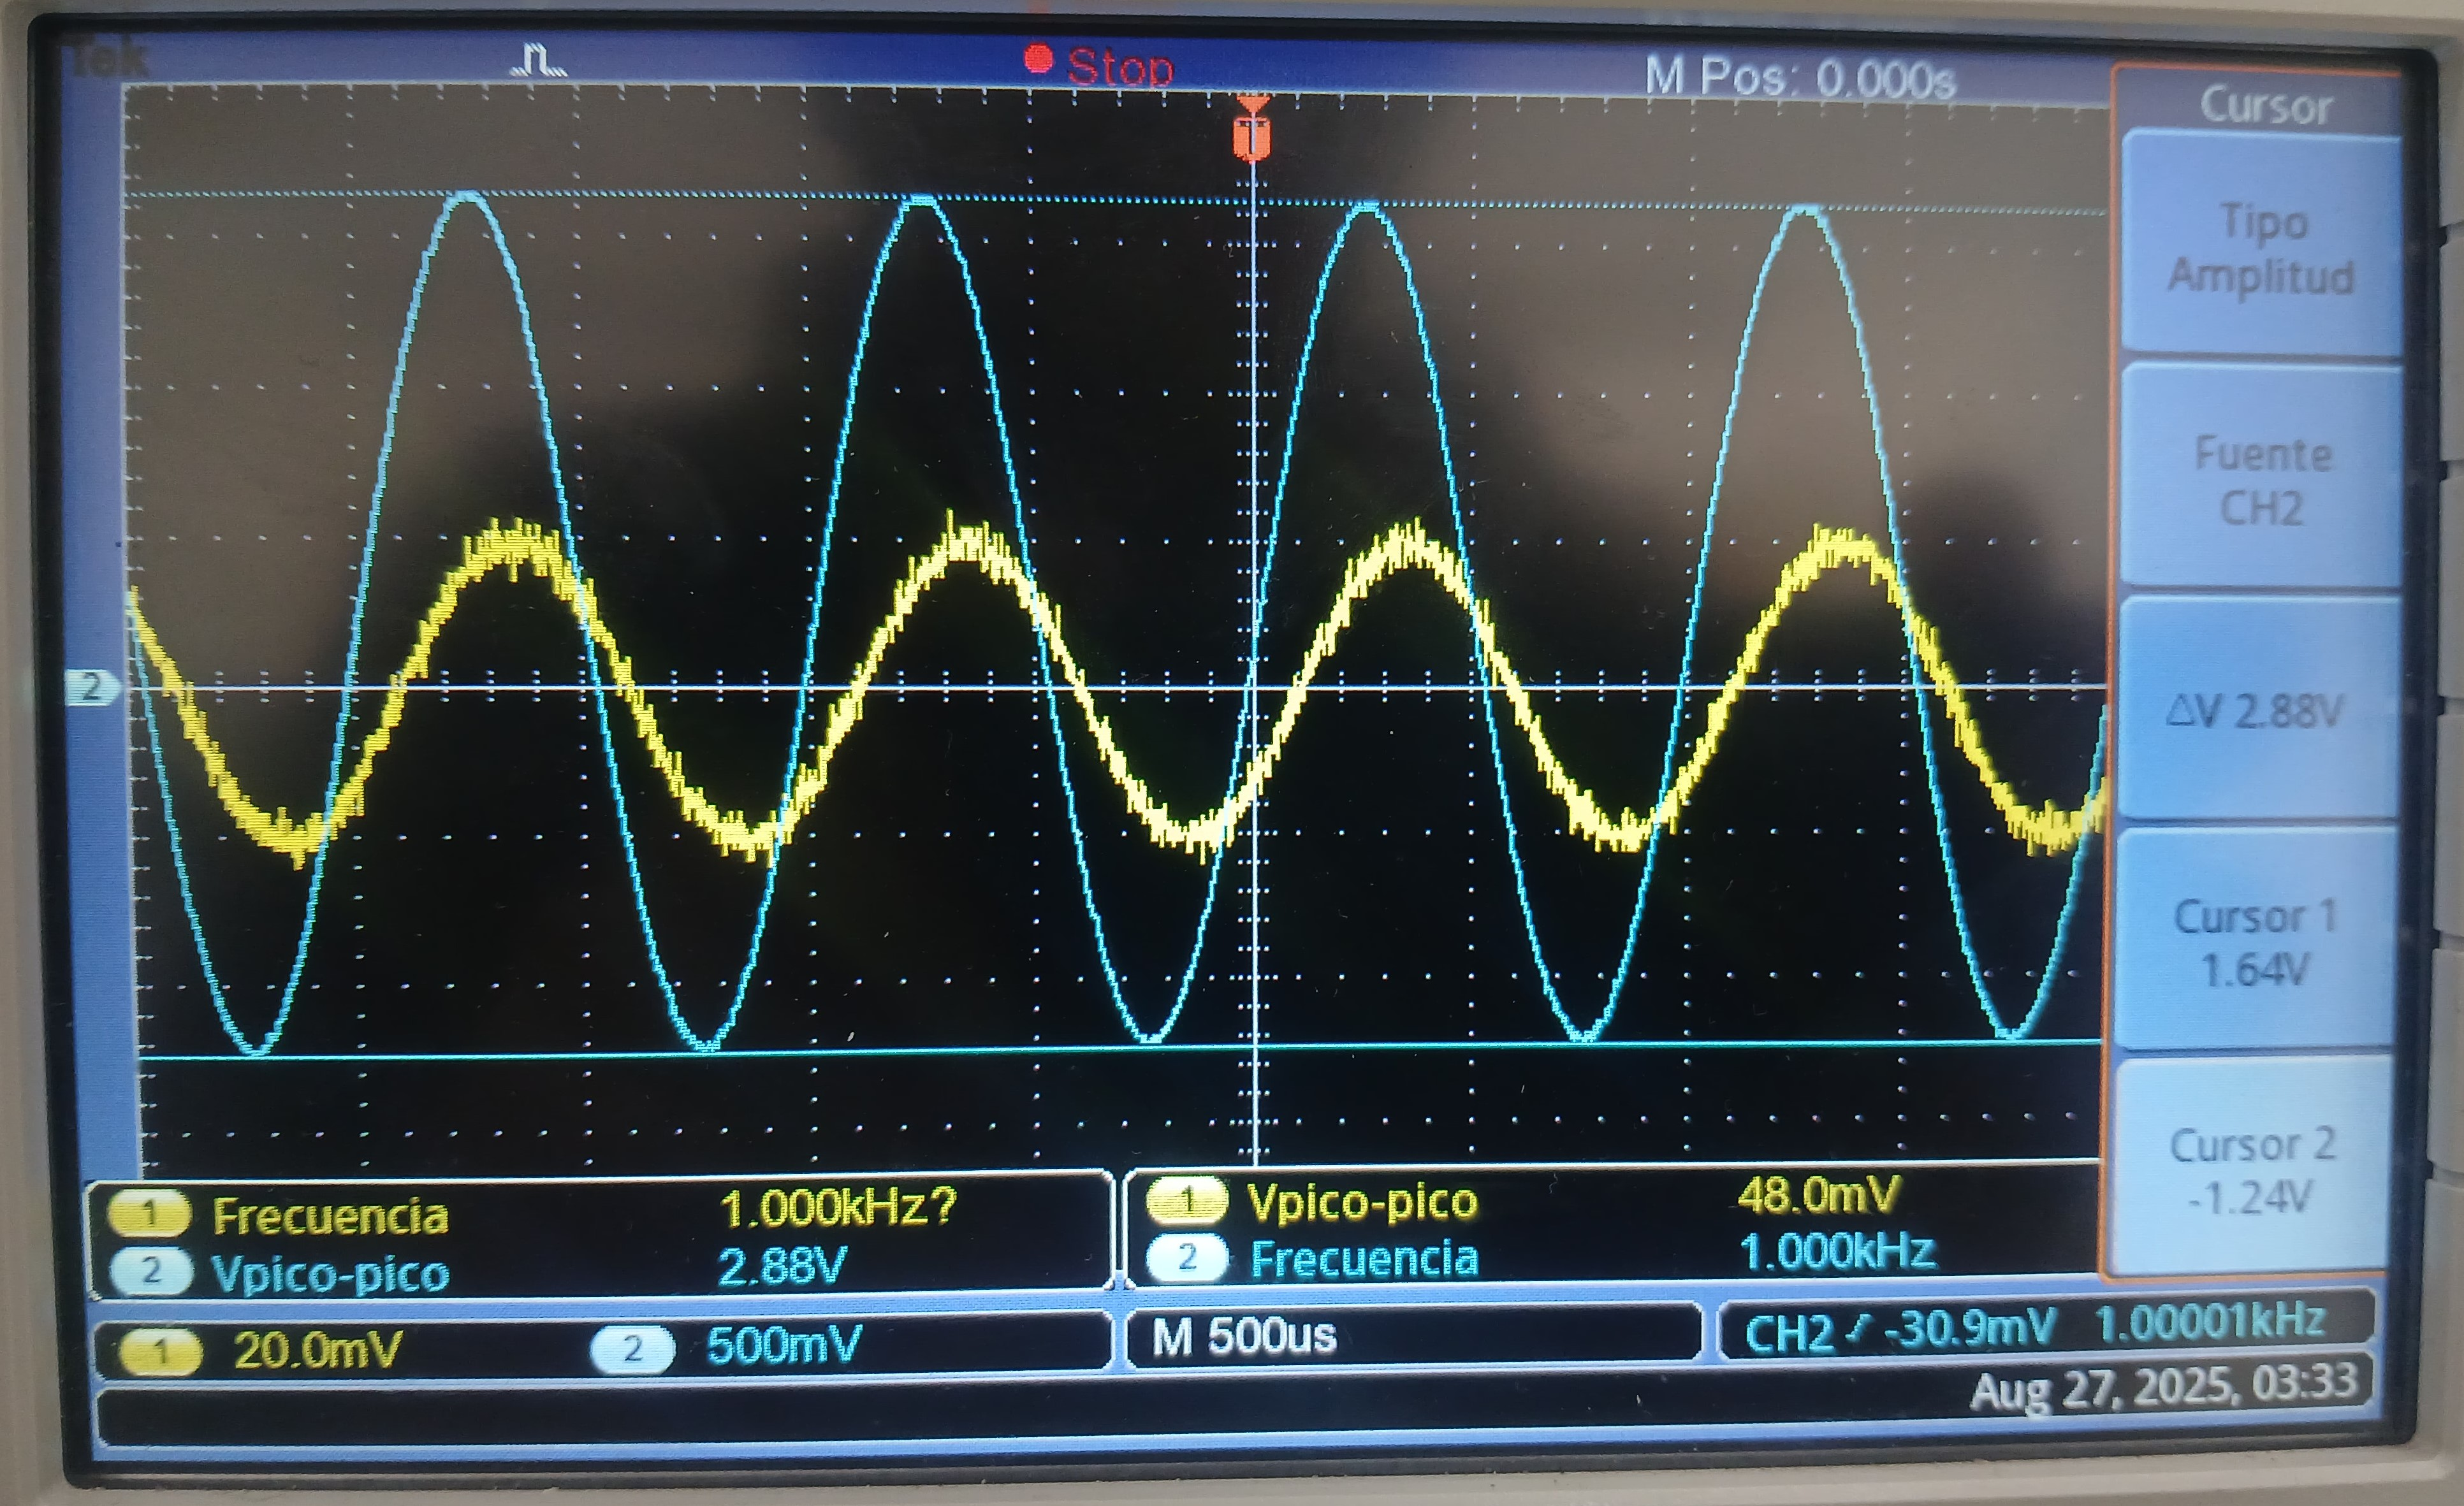
\includegraphics[width=0.5\textwidth]{media/offset-741}
	\caption{Medición Offset - Amplificador Operacional LM741}
	\label{fig:offset-741}
\end{figure}

Mediante este procedimiento como se puede apreciar en la figura \ref{fig:offset-741} la amplitud para el semiciclo positivo es de 1.64v y este mismo valor para el semiciclo negativo fue de 1.24v, por lo tanto se aprecia un offset de 0.40v que representa la diferencia entre los picos de la señal.

\section{Validación en el nivel de offset al variar el integrado LM741}

Una variación en el integrado para el mismo tipo de operacional confirmo que no existe un cambio significativo en el nivel de offset en la señal de salida encontrándose tal variación en el orden de las centésimas o del 10\% respecto al valor inicial, tales mediciones se pueden apreciar en la tabla.

% Please add the following required packages to your document preamble:
% \usepackage{multirow}
\begin{table}[]
	\centering
	\begin{tabular}{|ccccc|}
		\hline
		\multicolumn{5}{|c|}{\textbf{Niveles de offset - LM741}}                                                                                                                                                                \\ \hline
		\multicolumn{2}{|c|}{\textbf{Integrado}}                                 & \multicolumn{1}{c|}{\multirow{2}{*}{\textbf{Vmax}}} & \multicolumn{1}{c|}{\multirow{2}{*}{\textbf{Vmin}}} & \multirow{2}{*}{\textbf{Offset}} \\ \cline{1-2}
		\multicolumn{1}{|c|}{\textbf{N°}} & \multicolumn{1}{c|}{\textbf{Modelo}} & \multicolumn{1}{c|}{}                               & \multicolumn{1}{c|}{}                               &                                  \\ \hline
		\multicolumn{1}{|c|}{1}           & \multicolumn{1}{c|}{LM741}           & \multicolumn{1}{c|}{1,64}                           & \multicolumn{1}{c|}{-1,24}                          & 0,4                              \\ \hline
		\multicolumn{1}{|c|}{2}           & \multicolumn{1}{c|}{LM741}           & \multicolumn{1}{c|}{1,66}                           & \multicolumn{1}{c|}{-1,22}                          & 0,44                             \\ \hline
		\multicolumn{3}{|c|}{\textbf{Error estimado {[}\%{]}}}                                                                         & \multicolumn{2}{c|}{10}                                                                \\ \hline
	\end{tabular}
	\caption{Medición del offset para diferentes integrados - LM741}
	\label{tab:comparacion-offset-lm741}
\end{table}

Además el circuito utilizado para este propósito se muestra en la figura \ref{fig:implementacion-lm741} destacando que tal implementación se realizo de forma modular facilitando la evaluación para cada integrado.

\begin{figure}[h]
	\centering
	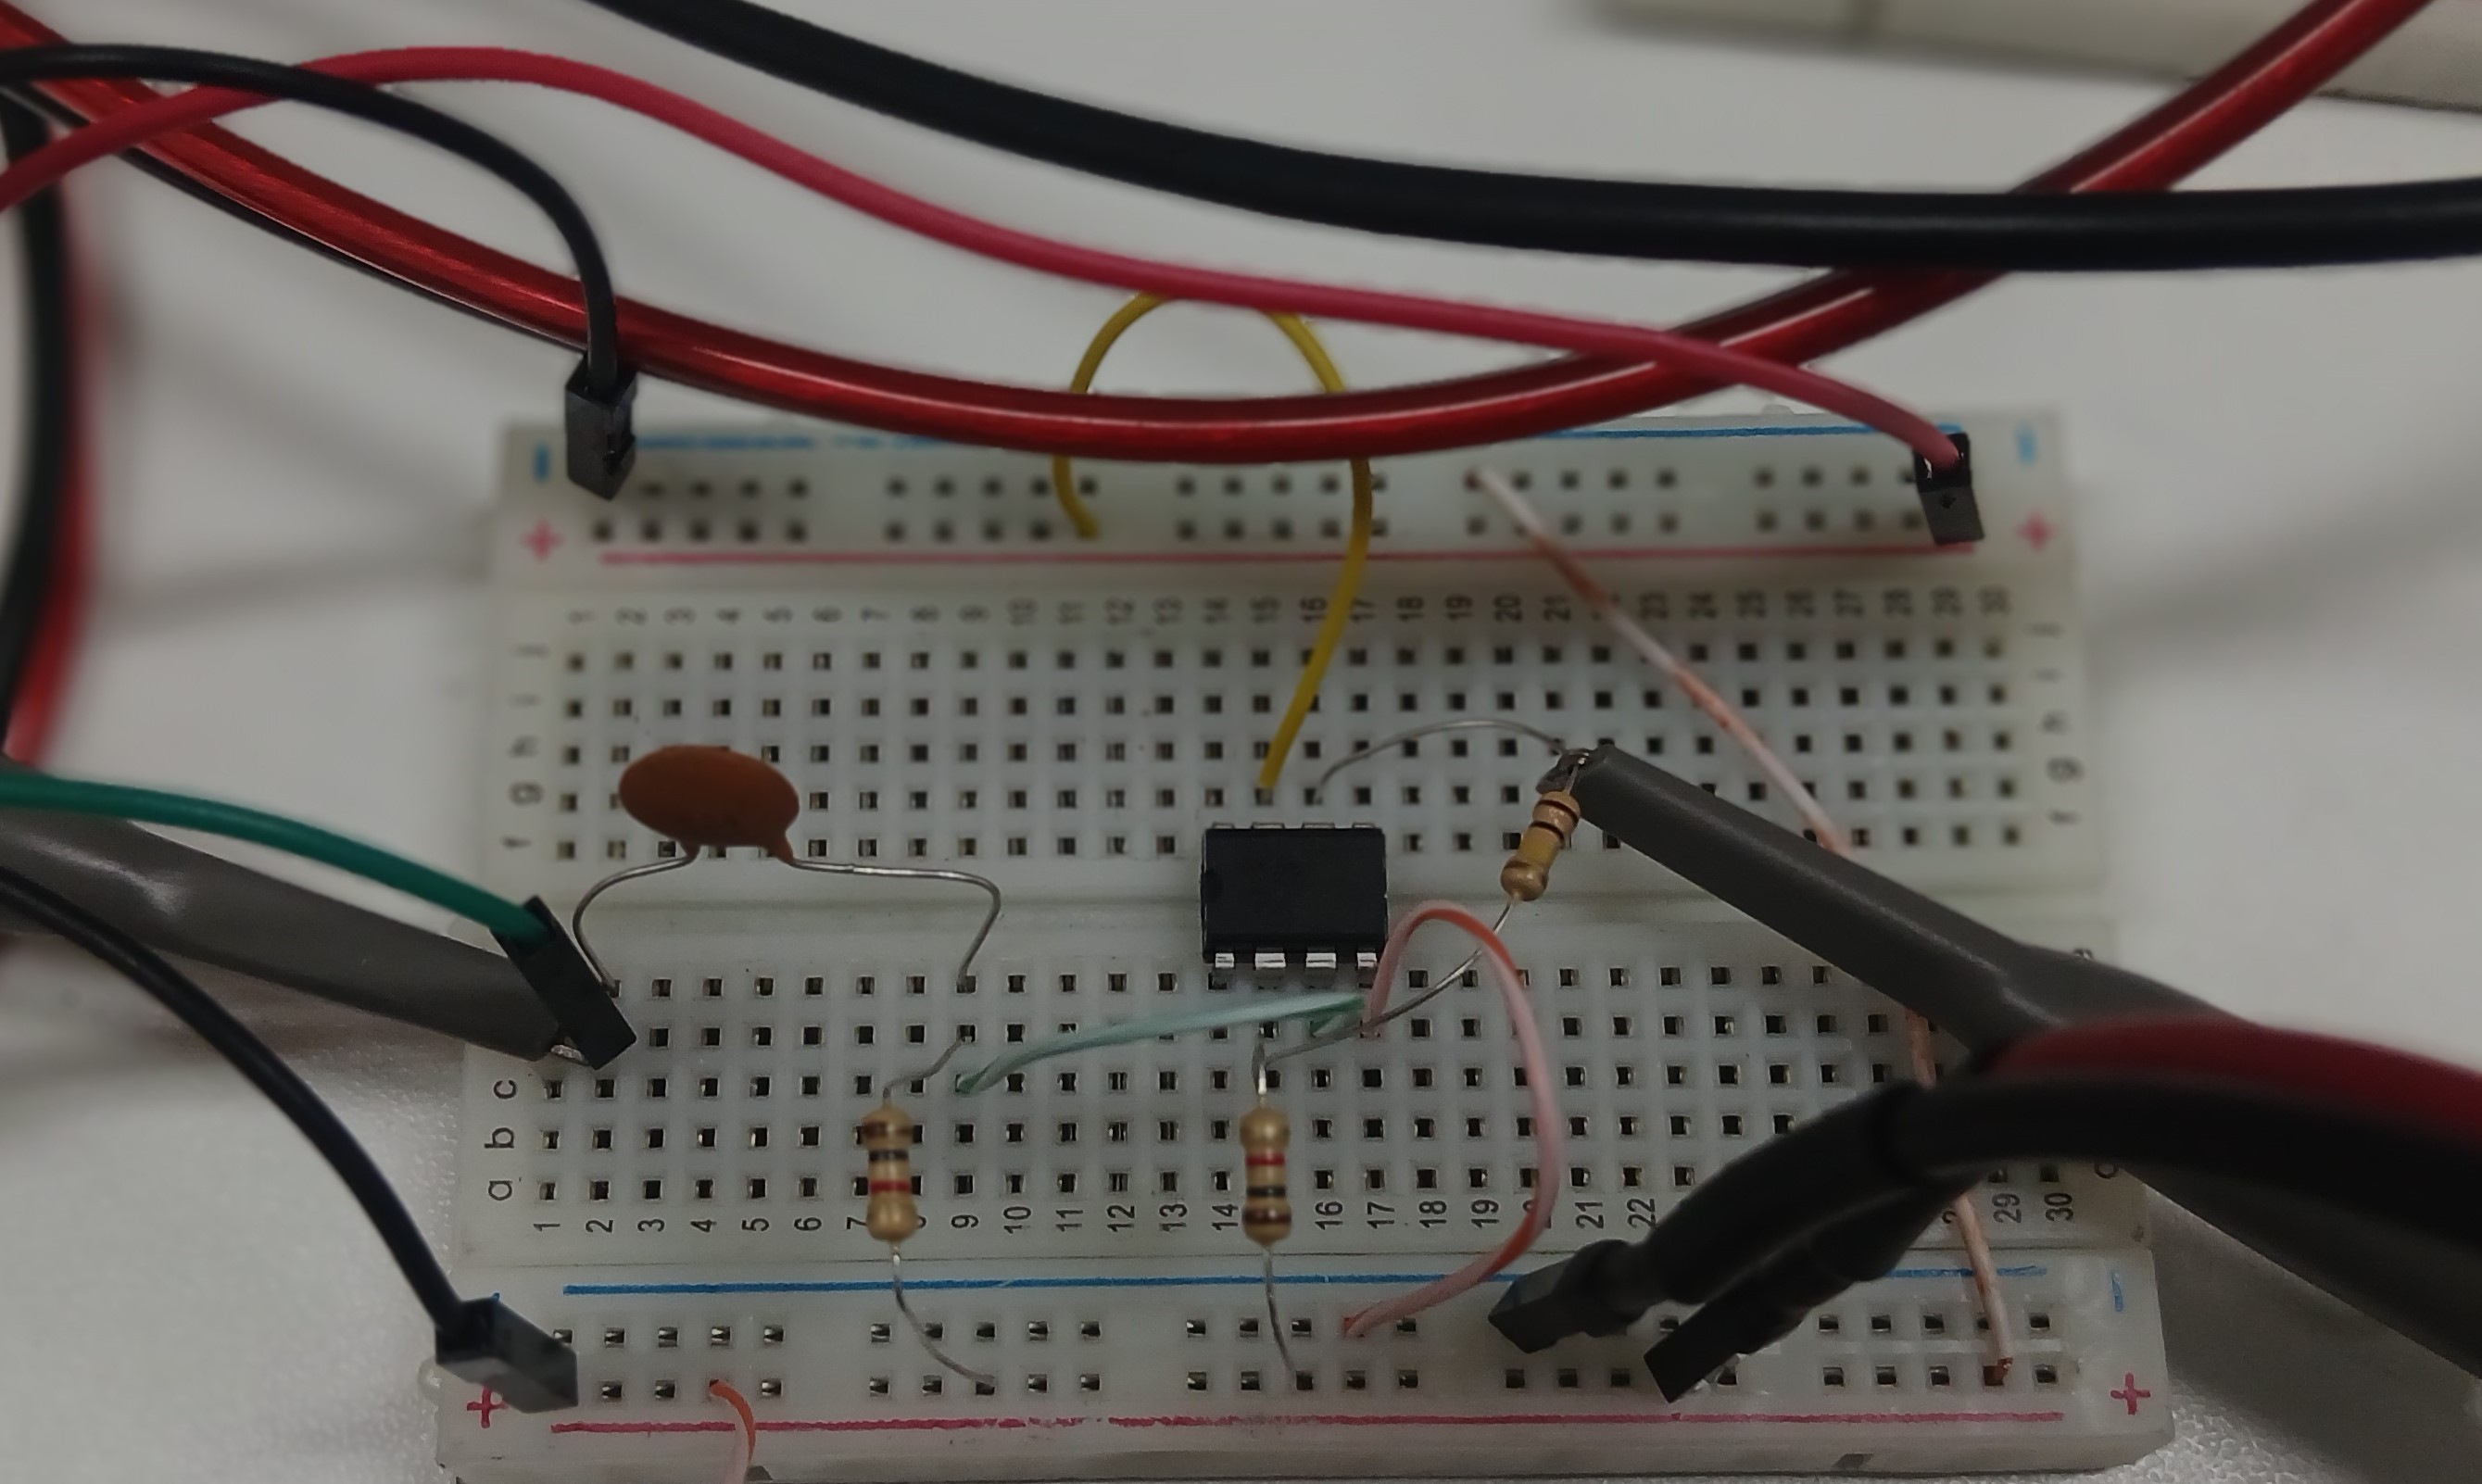
\includegraphics[width=0.5\textwidth]{media/implementacion-lm741}
	\caption{Implementación Amplificador no Inversor - LM741}
	\label{fig:implementacion-lm741}
\end{figure}

\subsection{¿Se encuentran dentro del rango según la hoja de datos del fabricante?}
Al verificar la hoja de datos del fabricante se puede apreciar que la variación para los niveles del offset del integrado oscilan entre los 1 - 5 mV para el modelo 741 y entre 2 a 6 mV para el modelo 741C.

Tal variación entre los niveles de offset para el integrado se muestra en la imagen \ref{fig:offset-datasheet-lm741} la cual además muestra los niveles de temperatura especificados para tal comportamiento respecto al offset en la salida.

\begin{figure}[h]
	\centering
	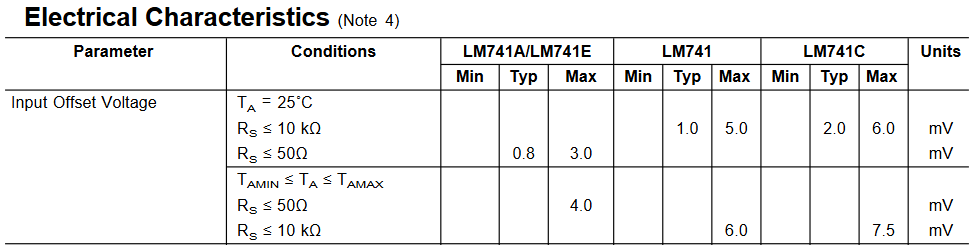
\includegraphics[width=0.8\textwidth]{media/offset-datasheet-lm741}
	\caption{Características Eléctricas del Integrado - LM741}
	\label{fig:offset-datasheet-lm741}
\end{figure}

\section{Amplificador no inversor con el amplificador operacional TL081}

Como se mostró en la figura \ref{fig:implementacion-lm741} la topologia permitió el cambio de tan solo el integrado para la validación y puesta en prueba de cada OPAM u amplificador operacional, obteniendo de esta forma los siguientes parámetros en la señal de salida.

\begin{itemize}
	\item Amplitud: 1.46 Vp
	\item Valor Medio (DC): -77.8 mV
	\item Valor RMS: 1.03 V
	\item Frecuencia: 1K Hz
\end{itemize}

Observando igualmente para el integrado TL081 un valor medio (DC) diferente de 0v lo cual indica la existencia de un nivel de offset siendo para este un voltaje negativo a causa del valor negativo observado.

\begin{figure}[h]
	\centering
	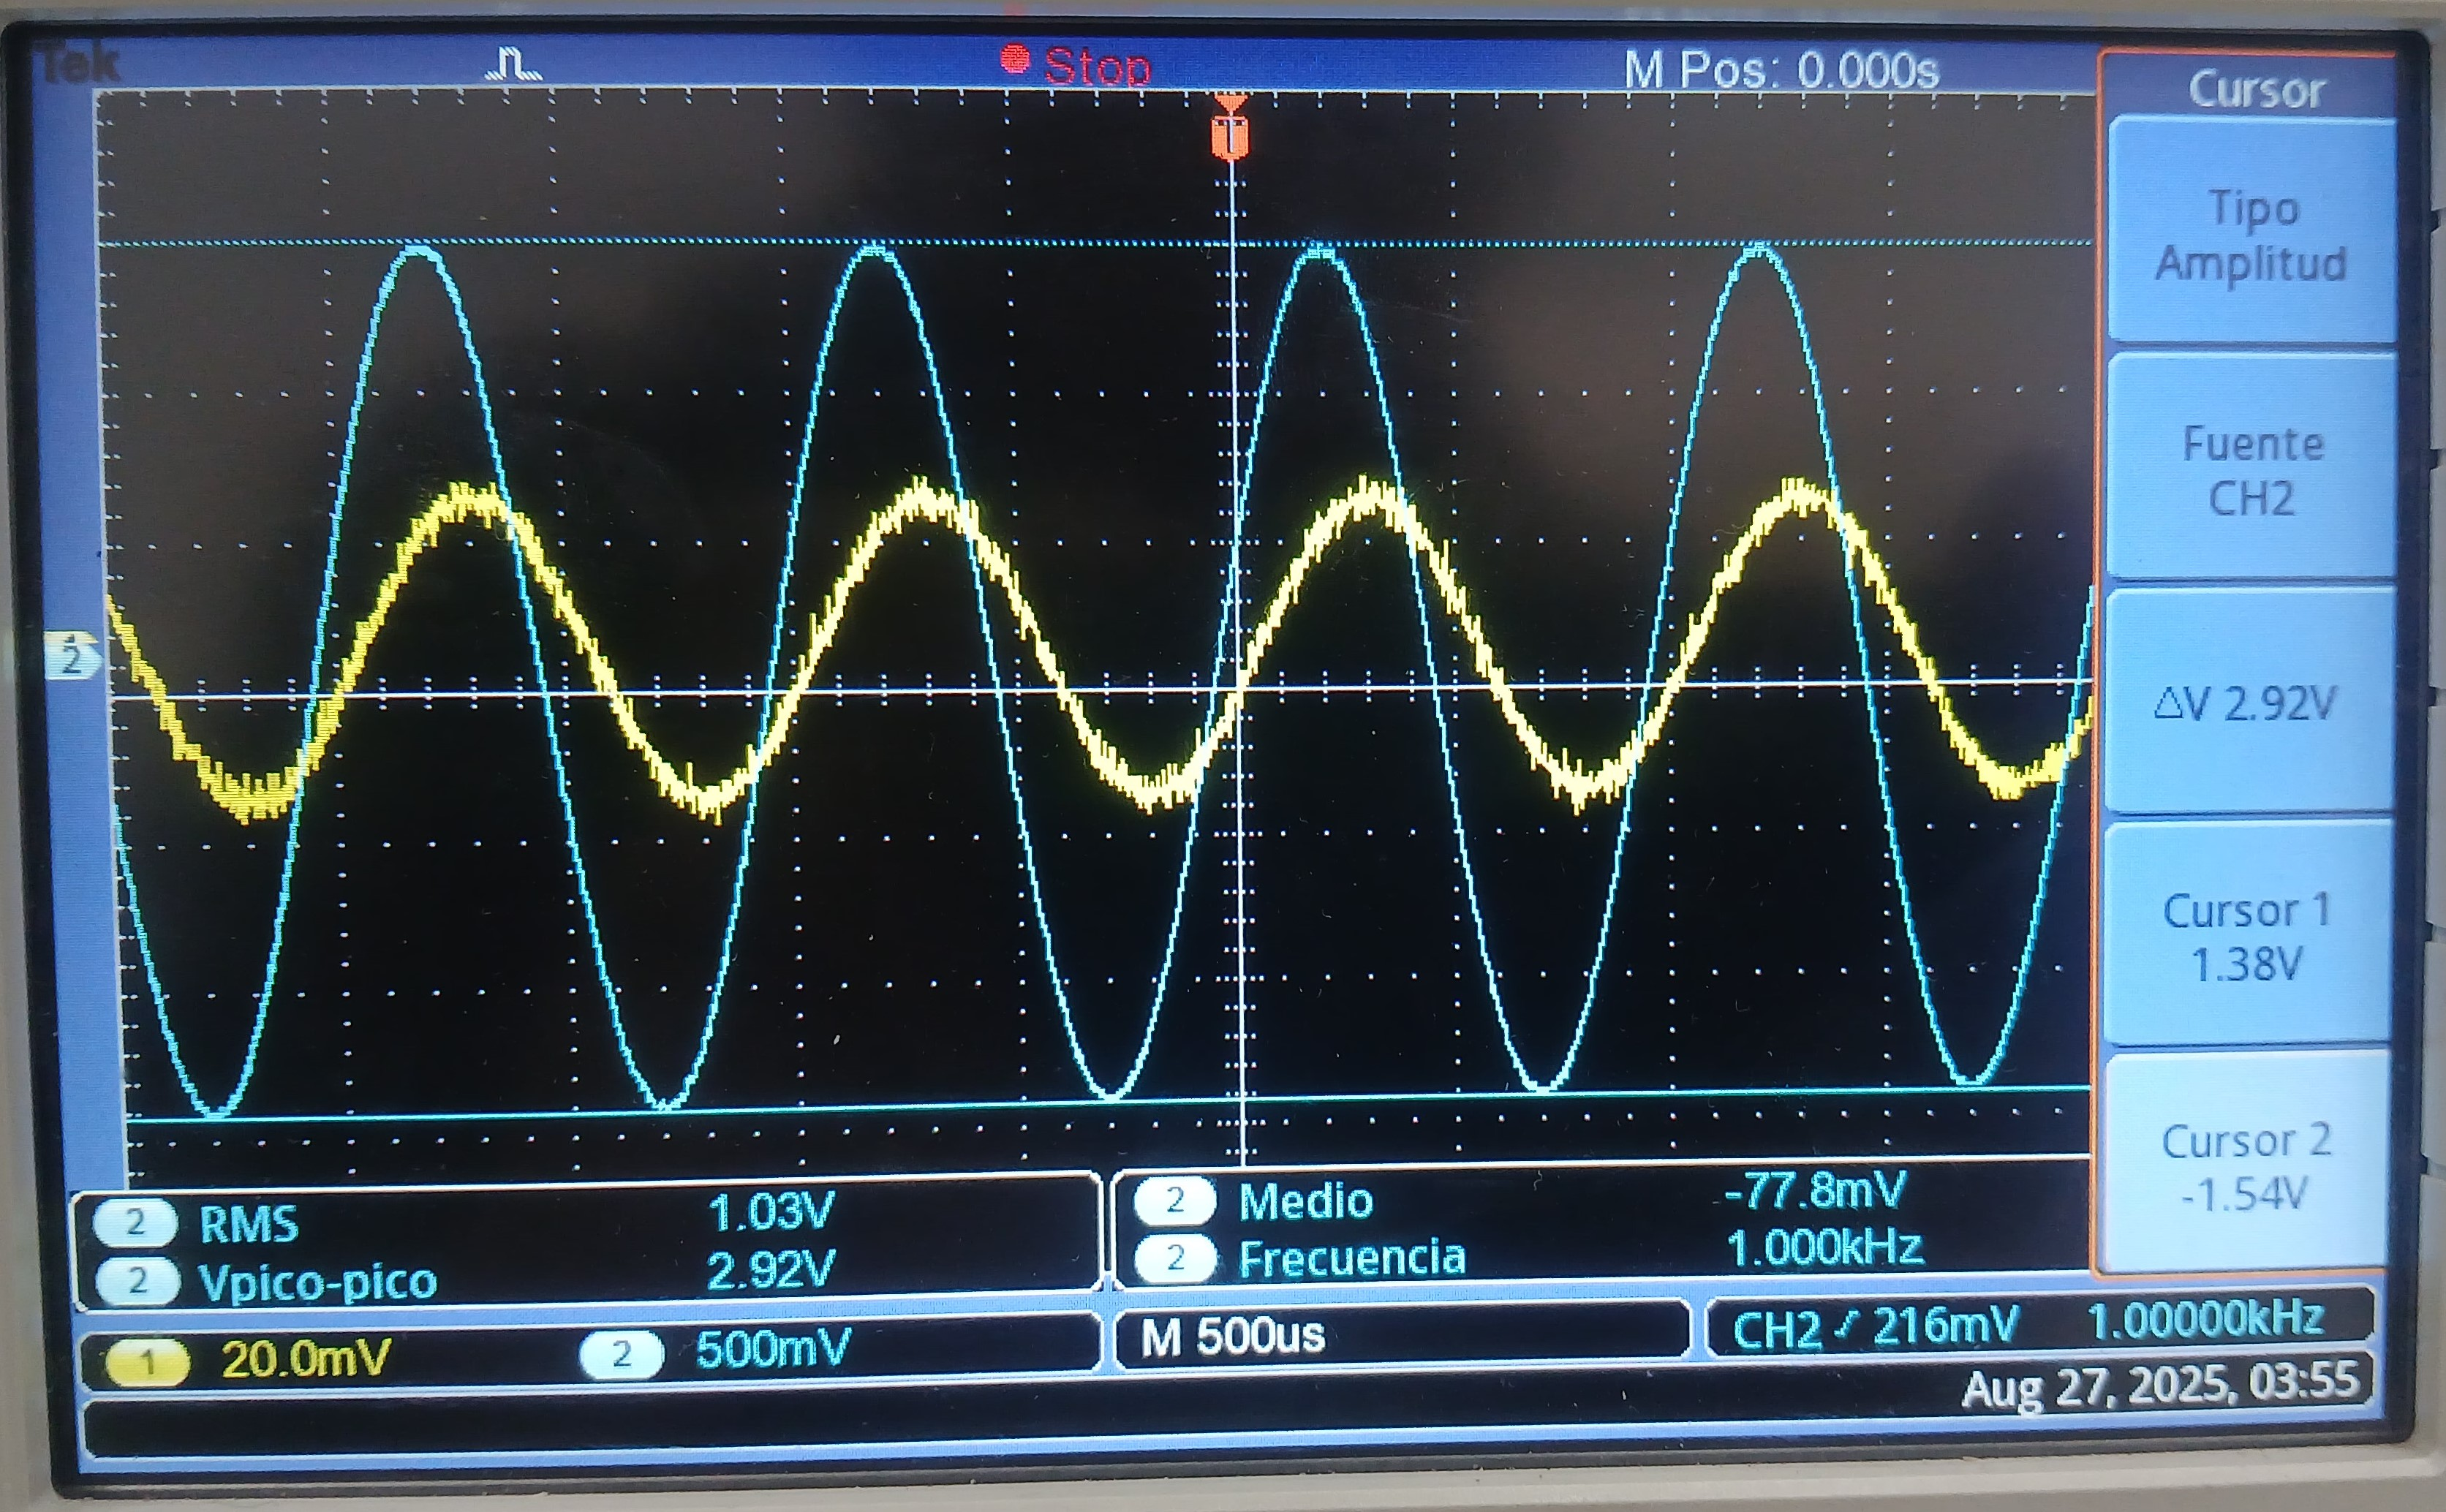
\includegraphics[width=0.5\textwidth]{media/offset-081}
	\caption{Nivel de Offset - TL081}
	\label{fig:offset-081}
\end{figure}

En la figura \ref{fig:offset-081} muestran el método de los cursos con los cuales se obtuvo el nivel de offset para este integrado, ubicándose la amplitud del semiciclo positivo en 1.38 V y para el semiciclo negativo de -1.54 V, confirmando un offset negativo de -0.16 V.

\section{Validación en el nivel de offset mediante la variación del TL081}

Las observaciones y pruebas realizadas para cada integrado se muestran en la tabla \ref{tab:offset-tl081} las cuales muestran una variación del 12.5\% entre integrados, destacando un error medianamente significativo entre encapsulados y el cual se debe tener en cuenta para aplicaciones que requieran de precisión en su salida.

\begin{table}[]
	\centering
	\begin{tabular}{|ccccc|}
		\hline
		\multicolumn{5}{|c|}{\textbf{Niveles de Offset - TL081}}                                                                                                                                                                \\ \hline
		\multicolumn{2}{|c|}{\textbf{Integrado}}                                 & \multicolumn{1}{c|}{\multirow{2}{*}{\textbf{Vmax}}} & \multicolumn{1}{c|}{\multirow{2}{*}{\textbf{Vmin}}} & \multirow{2}{*}{\textbf{Offset}} \\ \cline{1-2}
		\multicolumn{1}{|c|}{\textbf{N°}} & \multicolumn{1}{c|}{\textbf{Modelo}} & \multicolumn{1}{c|}{}                               & \multicolumn{1}{c|}{}                               &                                  \\ \hline
		\multicolumn{1}{|c|}{1}           & \multicolumn{1}{c|}{TL081}           & \multicolumn{1}{c|}{1,38}                           & \multicolumn{1}{c|}{-1,54}                          & 0,16                             \\ \hline
		\multicolumn{1}{|c|}{2}           & \multicolumn{1}{c|}{TL081}           & \multicolumn{1}{c|}{1,36}                           & \multicolumn{1}{c|}{-1,54}                          & 0,18                             \\ \hline
		\multicolumn{3}{|c|}{\textbf{Error estimado {[}\%{]}}}                                                                         & \multicolumn{2}{c|}{12.5}                                                              \\ \hline
	\end{tabular}
	\caption{Niveles de offset - TL081}
	\label{tab:offset-tl081}
\end{table}

\subsection{¿Se encuentran dentro del rango según la hoja de datos del fabricante?}
Al considerar los niveles de voltaje para el offset en la familia TL081 en la hoja de datos se puede destacar una relación de este valor respecto a la temperatura variación 18 V por cada grado por encima de los 25 C°, siendo así que para tal condición el offset medido y esperando se encontraría del rango definido.

\section{Anulación del offset para cada integrado}

Una forma de poder eliminar el nivel de offset es mediante el empleo de los pines de salida definidos por cada integrado y el uso de un potenciómetro como se muestra en \cite{National1998LM741} para el LM741 y \cite{TI_TL08x} para el integrado TL081, entre las terminales 1 y 5 que a su vez se encuentran referenciadas por el voltaje negativo $V_EE$.

En las figuras \ref{fig:offset-null-741} y \ref{fig:offset-null-081} se muestran la configuración a usar para el integrado LM741 y TL081 respectivamente.

\begin{figure}[h]
	\centering
	\begin{minipage}{0.3\linewidth}
		\centering
		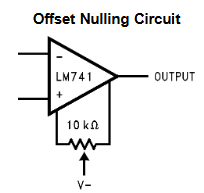
\includegraphics[width=\linewidth]{media/offset-null-741}
		\caption{Configuración null offset - LM741}
		\label{fig:offset-null-741}
	\end{minipage}
	\hfill
	\begin{minipage}{0.3\linewidth}
		\centering
		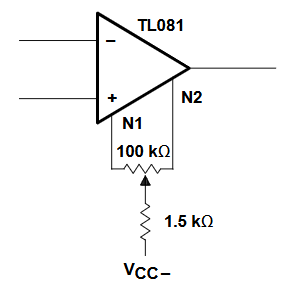
\includegraphics[width=\linewidth]{media/offset-null-081}
		\caption{Configuración null offset - TL081}
		\label{fig:offset-null-081}
	\end{minipage}
\end{figure} 

\begin{figure}[h]
	\centering
	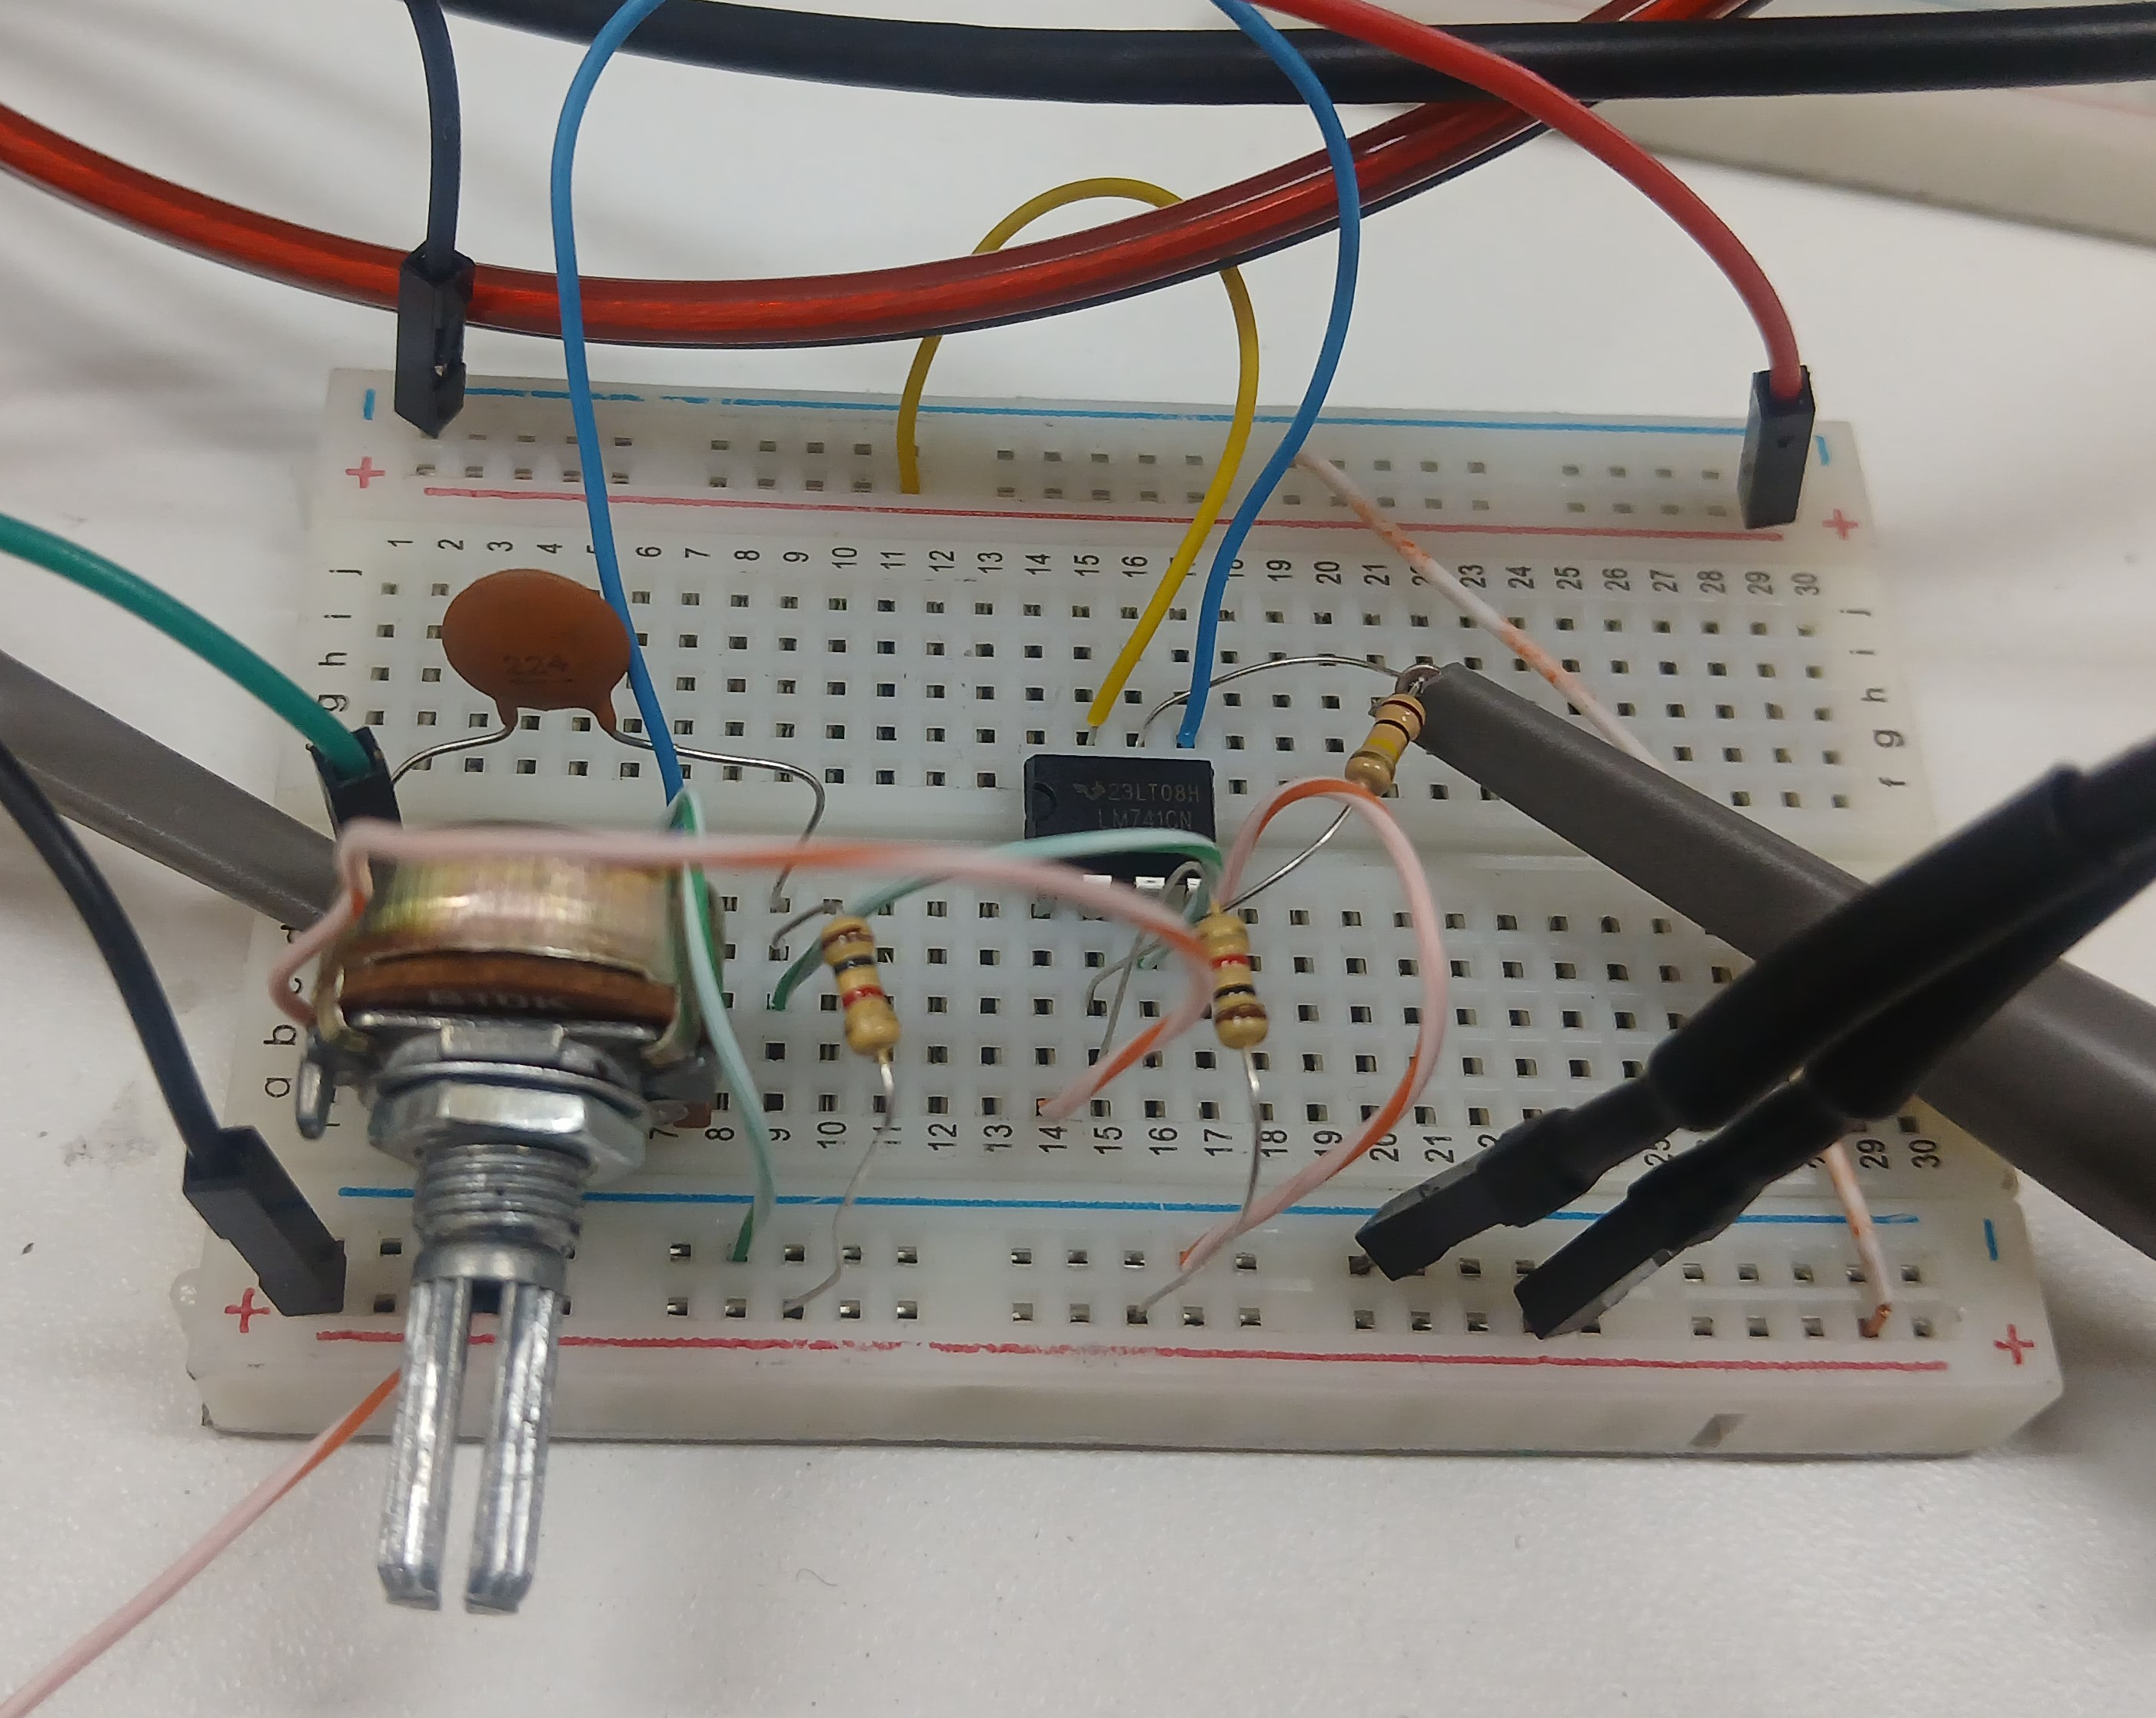
\includegraphics[width=0.4\textwidth]{media/implementacion-null-offset}
	\caption{Implementación null offset amplificadores operacionales}
	\label{fig:implementacion-null-offset}
\end{figure}

Tal configuración se aplico para poder eliminar el offset observado en cada integrado siendo la implementación del tal proceso observada en la figura \ref{fig:implementacion-null-offset}

La señal de salida luego de una calibración de la señal de salida mediante el potenciómetro se muestra en la figura \ref{fig:salida-offset-null} en el cual mediante el empleo de los cursores se estimaron los picos máximos para cada semiciclo obteniendo finalmente una igualdad entre ambos eliminando de esta forma el offset o componente DC en la señal.

\begin{figure}[h]
	\centering
	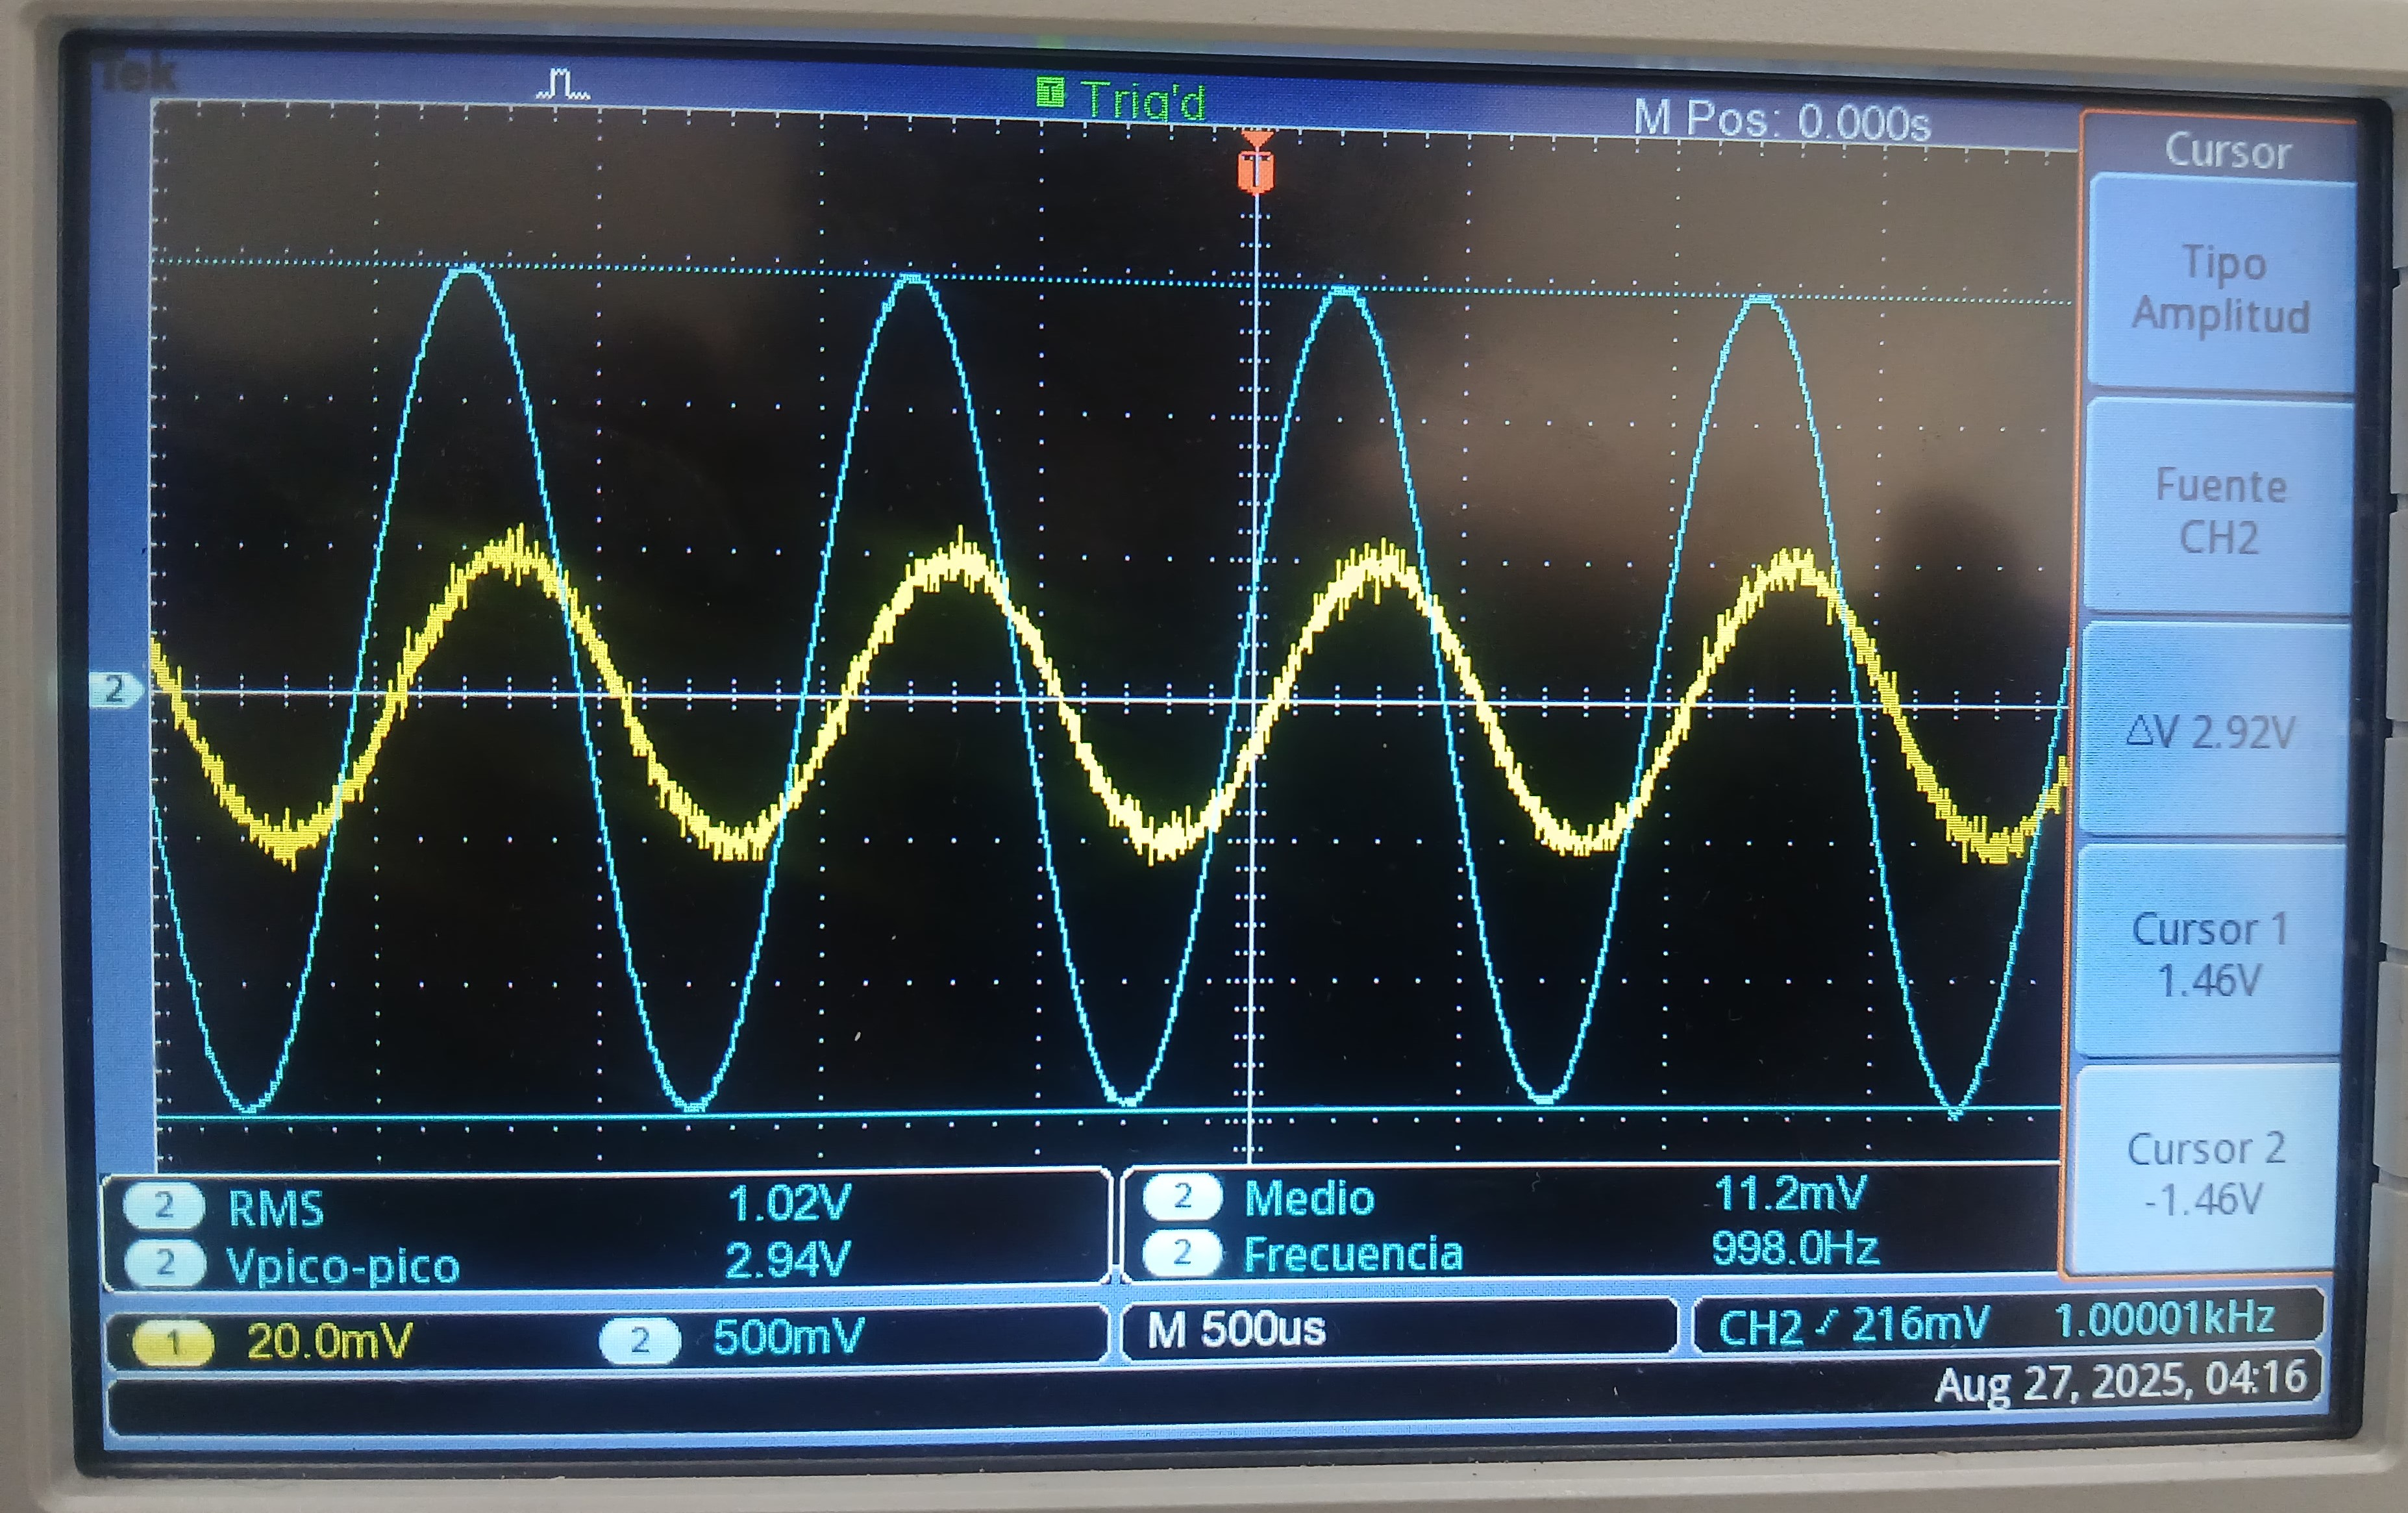
\includegraphics[width=0.4\textwidth]{media/salida-offset-null}
	\caption{Señal de salida - Eliminación del offset null}
	\label{fig:salida-offset-null}
\end{figure}


